\documentclass[12pt]{article}
\usepackage[english]{babel}
\usepackage{natbib}
\usepackage{url}
\usepackage[utf8x]{inputenc}
\usepackage{amsmath}
\usepackage{graphicx}
\graphicspath{{../docs/img/}}
\usepackage{parskip}
\usepackage{fancyhdr}
\usepackage{vmargin}
\usepackage{xcolor}
\usepackage{booktabs}
\usepackage{float}
\usepackage{pgfplots}
\usepackage{tikz}
\pgfplotsset{width=10cm,compat=1.9}

\setmarginsrb{3 cm}{2.5 cm}{3 cm}{2.5 cm}{1 cm}{1.5 cm}{1 cm}{1.5 cm}

\title{Sprint 6 Backlog}								% Title
\author{Thierry's Minions}								% Author
\date{12 Nov 2018}											% Date

\makeatletter
\let\thetitle\@title
\let\theauthor\@author
\let\thedate\@date
\makeatother

\pagestyle{fancy}
\fancyhf{}
\rhead{\theauthor}
\lhead{\thetitle}
\cfoot{\thepage}

\newcommand*{\userstory}[5][.25em]{
%  \begin{tabular*}{\maincolumnwidth}{l@{\extracolsep{\fill}}r}%
%    {\bfseries #2} & {\bfseries #4}\\%
%    {#3}\\%
%  \end{tabular*}%
%  \ifx&#5&%
%  \else{\\%
%    \begin{minipage}{\maincolumnwidth}%
%      #5%
%    \end{minipage}}\fi%
%  \par\addvspace{#1}
\textbf{#1} 
  }

\newcommand{\roundpic}[4][]{
  \tikz\node [circle, minimum width = #2,
    path picture = {
      \node [#1] at (path picture bounding box.center) {
        \includegraphics[width=#3]{#4}};
    }] {};}

\begin{document}

%%%%%%%%%%%%%%%%%%%%%%%%%%%%%%%%%%%%%%%%%%%%%%%%%%%%%%%%%%%%%%%%%%%%%%%%%%%%%%%%%%%%%%%%%

\begin{titlepage}
	\centering
    \vspace*{0.5 cm}
\roundpic[]{9cm}{9cm}{leader.jpg}

    \textsc{\LARGE Thierry's Minions/Team25\\[0.5em] Deliverable 5}\\[2.0 cm]	
	\textsc{\Large CSCC01 Fall 2018}\\[0.5 cm]				% Course Code
	\rule{\linewidth}{0.2 mm} \\[0.4 cm]
	{ \huge \bfseries \thetitle}\\
	\rule{\linewidth}{0.2 mm} \\[1.5 cm]
	
	\begin{minipage}{0.4\textwidth}
		\begin{flushleft} \large
			\emph{Submitted To:}\\
			Saba Kiaei\\
            Teaching Assistant\\
            Computer Science Department\\
			\end{flushleft}
			\end{minipage}~
			\begin{minipage}{0.4\textwidth}
            
			\begin{flushright} \large
			\emph{Submitted By :} \\
			Rishabh Kaant Sharma\\
            Joseph Sokolon\\
            Balaji Badu\\
            Jayden Arquelada\\
            Edgar Sarkisian\\
		\end{flushright}
        
	\end{minipage}\\[2 cm]
	
	
    
    
    
    
	
\end{titlepage}

%%%%%%%%%%%%%%%%%%%%%%%%%%%%%%%%%%%%%%%%%%%%%%%%%%%%%%%%%%%%%%%%%%%%%%%%%%%%%%%%%%%%%%%%%

\textcolor{black}{\tableofcontents}
\pagebreak

%%%%%%%%%%%%%%%%%%%%%%%%%%%%%%%%%%%%%%%%%%%%%%%%%%%%%%%%%%%%%%%%%%%%%%%%%%%%%%%%%%%%%%%%%

\section{Sprint Tasks}

\subsection{Task 6C: Create a GET endpoint which returns all the columns in a specific template.}
\begin{itemize}%
\item Story Points: 3
\item Template should be specified  in the header of request, with key template\_name.
\item Create a GET endpoint which returns all the columns in a specific template.
\item Data of columns should come from the TEMPLATES collection.
\end{itemize}

\subsection{Task 6F: Integrate and test feature.}
\begin{itemize}%
\item Story Points: 2
\item This task has a dependency on all previous tasks.
\item Ensure the integration between the server and client is working.
\item Test the entire feature and ensure it passes the conditions of acceptance.
\end{itemize}

\subsection{Task 7A: Create GET endpoint on server that returns population report data}
\begin{itemize}%
\item Story Points: 5
\item Create a GET endpoint which returns all the Data needed for the population report.
\item Age distribution for all groups will be below 30, 30 -49, over 49
\item A) Distribution of age from needs \& assessments Referrals  (Pie chart)
\item B) Distribution of age from employment services (Pie chart)	
\item C) Distribution of age from language (Pie chart)
\item D) From all three, the percentage of people who have children (Bar Graph)
\end{itemize}

\subsection{Task 7B: Add population report to Client.}
\begin{itemize}%
\item Story Points: 3
\item This task has a dependency on task 7A.
\item Add button to Report Generation screen for population report.
\item Add controller to make request to server for population report.
\item Generate report into PDF and send it to user.
\end{itemize}

\subsection{Task 8A: Add Ui for Conflicts to Client}
\begin{itemize}%
\item Story Points: 3
\item Create UI to display invalid rows of the conflict.
\item Create controller to get conflict data from server.
\item Create controller to send conflict resolution to server.
\item If there is no conflicts display text. All Conflicts Resolved!
\end{itemize}


\subsection{Task 8B: Change insert row method on server to handle conflicts}
\begin{itemize}%
\item Story Points: 5
\item Change insert row method on server to handle conflicts.
\item If there is a conflict create a conflict document in CONFLICTS collection.
\end{itemize}

\subsection{Task 8C: Create GET endpoint on server that returns a conflict}
\begin{itemize}%
\item Story Points: 3
\item Create GET endpoint on server that returns a conflict.
\item Should only send a single conflict, order doesn't matter.
\item If no conflicts exist send an empty object.
\end{itemize}

\subsection{Task 8C: Create POST endpoint on server that resolves a conflict}
\begin{itemize}%
\item Story Points: 3
\item Create POST endpoint on server that resolves a conflict
\item Resolution to conflict will be in body of request. 
\item Delete the conflict document from conflicts collection.
\item Add the resolution back in the corresponding template.
\end{itemize}

\subsection{Task 8E: Integrate and test feature.}
\begin{itemize}%
\item Story Points: 5
\item This task has a dependency on all previous tasks.
\item Ensure the integration between the server and client is working.
\item Test the entire feature and ensure it passes the conditions of acceptance.
\end{itemize}

\subsection{Task 9A: Create data for all possible values of columns}
\begin{itemize}%
\item Story Points: 2
\item More data needs to be added to the template based on what the possible values for those columns can be.
\end{itemize}

\subsection{Task 9B: Create UI for Trend Reports Screen}
\begin{itemize}%
\item Story Points: 3
\item Create a trends UI where the user can choose columns for which they would like to see the trends. 
\end{itemize}

\subsection{Task 9C: Create GET endpoint on server for all possible values in a column}
\begin{itemize}%
\item Story Points: 3
\item This task has a dependency on task 9A
\item Create GET endpoint on server which returns all possible values in a column
\end{itemize}

\subsection{Task 9D: Create GET endpoint on server for data for a specified column}
\begin{itemize}%
\item Story Points: 2
\item Create GET endpoint on server which returns the current data on a specific column from database.
\end{itemize}

\subsection{Task 9E: Create controllers in Client}
\begin{itemize}%
\item Story Points: 3
\item Create controller to get all possible data values in a column from server.
\item Create controller to get all current data values in a column from server.
\item Create controller to generate the data into a pdf report.
\end{itemize}

\newpage
\section{Sprint Plan}

\textbf{Sprint 6 : November 19th - November 25th (Monday - Sunday)}
\begin{table}[H]
\begin{tabular}{@{}c|c|c|c|ccccccc@{}}
\toprule
Story & Task & Dependency & \begin{tabular}[c]{@{}c@{}}Story\\ Points\end{tabular} & \begin{tabular}[c]{@{}c@{}}Day\\ 1\end{tabular} & \begin{tabular}[c]{@{}c@{}}Day\\ 2\end{tabular} & \begin{tabular}[c]{@{}c@{}}Day \\ 3\end{tabular} & \begin{tabular}[c]{@{}c@{}}Day \\ 4\end{tabular} & \begin{tabular}[c]{@{}c@{}}Day \\ 5\end{tabular} & \begin{tabular}[c]{@{}c@{}}Day \\ 6\end{tabular} & \begin{tabular}[c]{@{}c@{}}Day \\ 7\end{tabular} \\ \midrule
6     & C    &            & 3                                                      & BB:3                                            &                                                 &                                                  &                                                  &                                                  &                                                  &                                                  \\
6     & F    & ALL        & 2                                                      &                                                 &                                             &                                                      &                                                  & JS:2                                             &                                                  &                                                  \\
7     & A    &            & 5                                                      &                                                 &  JS:5                                           &                                                  &                                                  &                                                  &                                                  &                                                  \\
7     & B    & A          & 3                                                      &                                                 &                                                 & JA:3                                             &                                                  &                                                  &                                                  &                                                  \\
8     & A    &            & 3                                                      & JA:3                                            &                                                 &                                                  &                                                  &                                                  &                                                  &                                                  \\
8     & B    &            & 5                                                      & ES:5                                            &                                                 &                                                  &                                                  &                                                  &                                                  &                                                  \\ 
8     & C    &            & 3                                                      &                                                 &                                                 &                                                  &  BB:3                                            &                                                  &                                                  &                                                  \\ 
8     & D    &            & 3                                                      &                                                 &                                                 & JS:3                                             &                                                  &                                                  &                                                  &                                                  \\ 
8     & E    & All        & 5                                                      &                                                 &                                                 &                                                  &                                                  &  ES:5                                            &                                                  &                                                  \\ 
9     & A    &            & 2                                                      &                                                 &  RS:2                                           &                                                  &                                                  &                                                  &                                                  &                                                  \\ 
9     & B    &            & 3                                                      &                                                 &                                                 & RS:3                                             &                                                  &                                                  &                                                  &                                                  \\ 
9     & C    & A          & 3                                                      &                                                 &                                                 &                                                  &                                                  &  RS:3                                                &                                                  &                                                  \\ 
9     & D    &            & 2                                                      &                                                 &                                                 &                                                  &                                                  &  RS:2                                                 &                                                  &                                                  \\ 
9     & E    &            & 3                                                      &                                                 &                                                 &                                                  &                                                  &                                                  &  RS:3                                                &                                                  \\ \bottomrule
\end{tabular}
\end{table}

\begin{itemize}%
\item Estimated story points team can complete: 45
\item The team believes they can complete User Story's 6, 7, \& 8 by end of day 5, \& User Story 9 by end of the day 6. 
\end{itemize}

\newpage

\section{Sprint Report}

\textbf{Sprint 6 : November 19th - November 25th (Monday - Sunday)}
\begin{table}[H]
\begin{tabular}{@{}c|c|c|c|ccccccc@{}}
\toprule
Story & Task & Dependency & \begin{tabular}[c]{@{}c@{}}Story\\ Points\end{tabular} & \begin{tabular}[c]{@{}c@{}}Day\\ 1\end{tabular} & \begin{tabular}[c]{@{}c@{}}Day\\ 2\end{tabular} & \begin{tabular}[c]{@{}c@{}}Day \\ 3\end{tabular} & \begin{tabular}[c]{@{}c@{}}Day \\ 4\end{tabular} & \begin{tabular}[c]{@{}c@{}}Day \\ 5\end{tabular} & \begin{tabular}[c]{@{}c@{}}Day \\ 6\end{tabular} & \begin{tabular}[c]{@{}c@{}}Day \\ 7\end{tabular} \\ \midrule
6     & C    &            & 3                                                      & BB:3                                            &                                                 &                                                  &                                                  &                                                  &                                                  &                                                  \\
6     & F    & ALL        & 2                                                      &                                                 &                                                &                                                   &                                                  &                                                  &  JS:3                                                &  JS:2                                                \\
7     & A    &            & 5                                                      &                                                 &                                             &                                                  &                                                  &                                                  &  JS:5                                                &                                                  \\
7     & B    & A          & 3                                                      &                                                 &                                                 &                                                 &                                                  &                                                  &                                                  & JA:3                                                 \\
8     & A    &            & 3                                                      & JA:5                                            &                                                 &                                                  &                                                  &                                                  &                                                  &                                                  \\
8     & B    &            & 5                                                      & ES:3                                            &                                                 &                                                 &   ES:3                                                &                                                  &                                                  &                                                  \\ 
8     & C    &            & 3                                                      &                                                 &                                                 &                                                  &                                              &         BB:3                                         &                                                  &                                                  \\ 
8     & D    &            & 3                                                      &                                                 &                                                 &                                                  &                                                  &    JS:3                                              &                                                  &                                                  \\ 
8     & E    & All        & 5                                                      &                                                 &                                                 &                                                  &                                                  &                                            &   ES:5                                                 &                                                  \\ 
9     & A    &            & 2                                                      &                                                 &  RS:2                                           &                                                  &                                                  &                                                  &                                                  &                                                  \\ 
9     & B    &            & 3                                                      &                                                 &                                                 & RS:3                                             &                                                  &                                                  &                                                  &                                                  \\ 
9     & C    & A          & 3                                                      &                                                 &                                                 &                                                  &                                                  &  RS:3                                                &                                                  &                                                  \\ 
9     & D    &            & 2                                                      &                                                 &                                                 &                                                  &                                                  &  RS:2                                                 &                                                  &                                                  \\ 
9     & E    &            & 3                                                      &                                                 &                                                 &                                                  &                                                  &                                                  &  RS:3                                                &                                                  \\ \bottomrule
\end{tabular}
\end{table}
\begin{itemize}%
\item Actual story points burned: 45
\item The team completed User Story 8 \& 9 on day 6 of the sprint. 
\item The team completed User Story 6 \& 7 on day 7 of the sprint. 
\end{itemize}

\section{Sprint Burndown Chart}

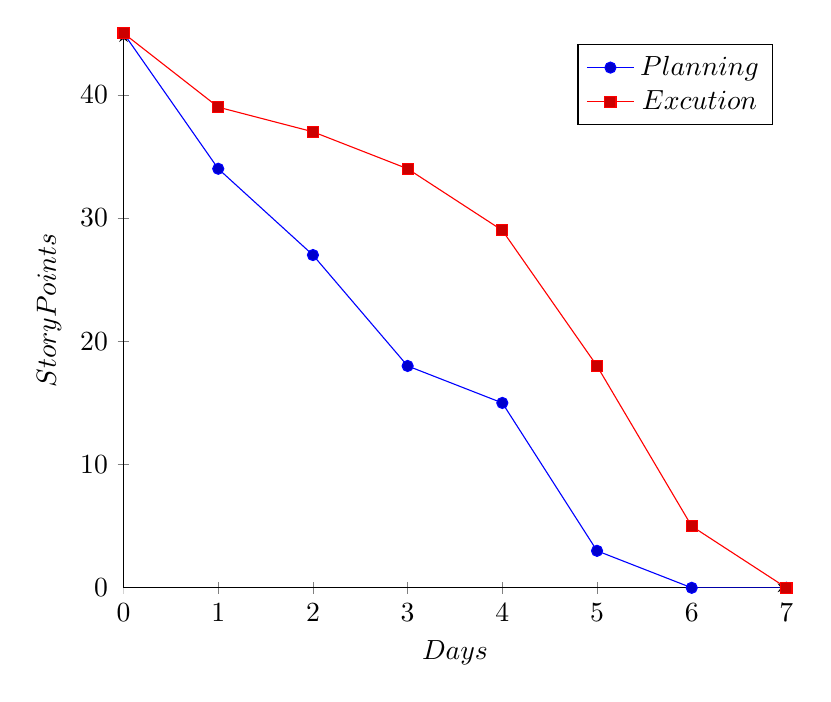
\begin{tikzpicture}
\begin{axis}[
    axis lines = left,
    xlabel = $Days$,
    ylabel = {$Story Points$},
]
\addplot coordinates {(0,45) (1,34) (2,27) (3,18) (4,15) (5,3) (6,0) (7,0)};
\addlegendentry{$Planning$}
\addplot coordinates {(0,45) (1,39) (2,37) (3,34) (4,29) (5,18) (6,5) (7,0)};
\addlegendentry{$Excution$}
\end{axis}
\end{tikzpicture}

\newpage
\bibliographystyle{plain}
\bibliography{biblist}

\end{document}